%%%%%%%%%%%%%%%%%%%%%%%%%%%%%%%%%%%%%%%%%%%%%%%%
%\newpage
Application of the Zoloratarev problems are presented here. In  \cref{ssec:filter_iir}, we consider the infinite impulse response (IIR) filter design problem. 

\subsection{IIR digital filter design (Z4)}\label{ssec:filter_iir}

We are interested in designing a bandpass filter (for simplicity, we restrict the exposition to this class of filter but multi-band can easily be obtained). The problem consists in designing a filter which amplitude is $1$ over the frequencies of interest ($F$ set) and $\epsilon>0$ over the frequencies  to be discarded ($E$ set). This is precisely the Z4 sign problem. To apply the methodology presented, following steps are chosen\footnote{Filter and figures can be obtained with \texttt{demo3\_filterDesign.m}.}:
\begin{itemize}
\item Define $E$ ($=\epsilon$) and $F$ ($=1$) as
$$
\begin{array}{rcl}
E &=& e^{\imath \pi \Theta_1} \cup e^{\imath \pi \Theta_3} \\
F &=& e^{\imath \pi \Theta_2}
\end{array}
$$
with $\Theta_1=[10^{-3},0.1]$,  $\Theta_2=[0.3,0.4]$ and $\Theta_1=[0.6,0.9]$ sets. In the following application each set is linearly sampled between bounds with 50, 100 and 50 points. Refer to \cref{fig:filter} (left) to view the $E$ (grey dots) and $F$ (black dots) sets, and to \cref{fig:filter} (right) to view the corresponding values in Bode like form (blue dots).
\item  Then, apply the LF approach, as exposed in the main document. Here, as we seek for a digital filter that can be effectively implemented on a real-time system, real entries i nthe coefficients are expected only. Therefore, interpolation points $E\cup F$ are closed by conjugation before applying LF with the modification explained in \cite[\S 2.4.5]{ali17}. This is why on \cref{fig:filter} (right), data are both on positive and negative sides. The LF computes the order with a singular value threshold set to $10^{-12}$, and a very low  Z3 approximation metric $\sigma_r$ is reached, see  \cref{fig:filter} (left). Now the rational approximant $\mathbf h_4$ has real-valued coefficients only and both poles and zeros come closed by conjugation.
\item As revealed by the \cref{fig:filter} (left), some poles $p(\mathbf h_4)$ of the rational approximant are outside the unit circle $\mathcal C(0,1)$ (solid black line), which results in an unstable rational function, not implementable. Here, we chose to project the unstable poles inside the unit circle to preserve the gain. However, this indirectly impacts the phase in an uncontrollable manner, as shown in \cref{fig:filter} (right-bottom). 
\item As the coefficients are real, both the transfer function and realization are real. It is finally possible to create dynamical system with sampling time $T_s$ and to run it in real-time (see \cref{fig:filter_td}).
\end{itemize}

\begin{figure}[ht]
    \centering
    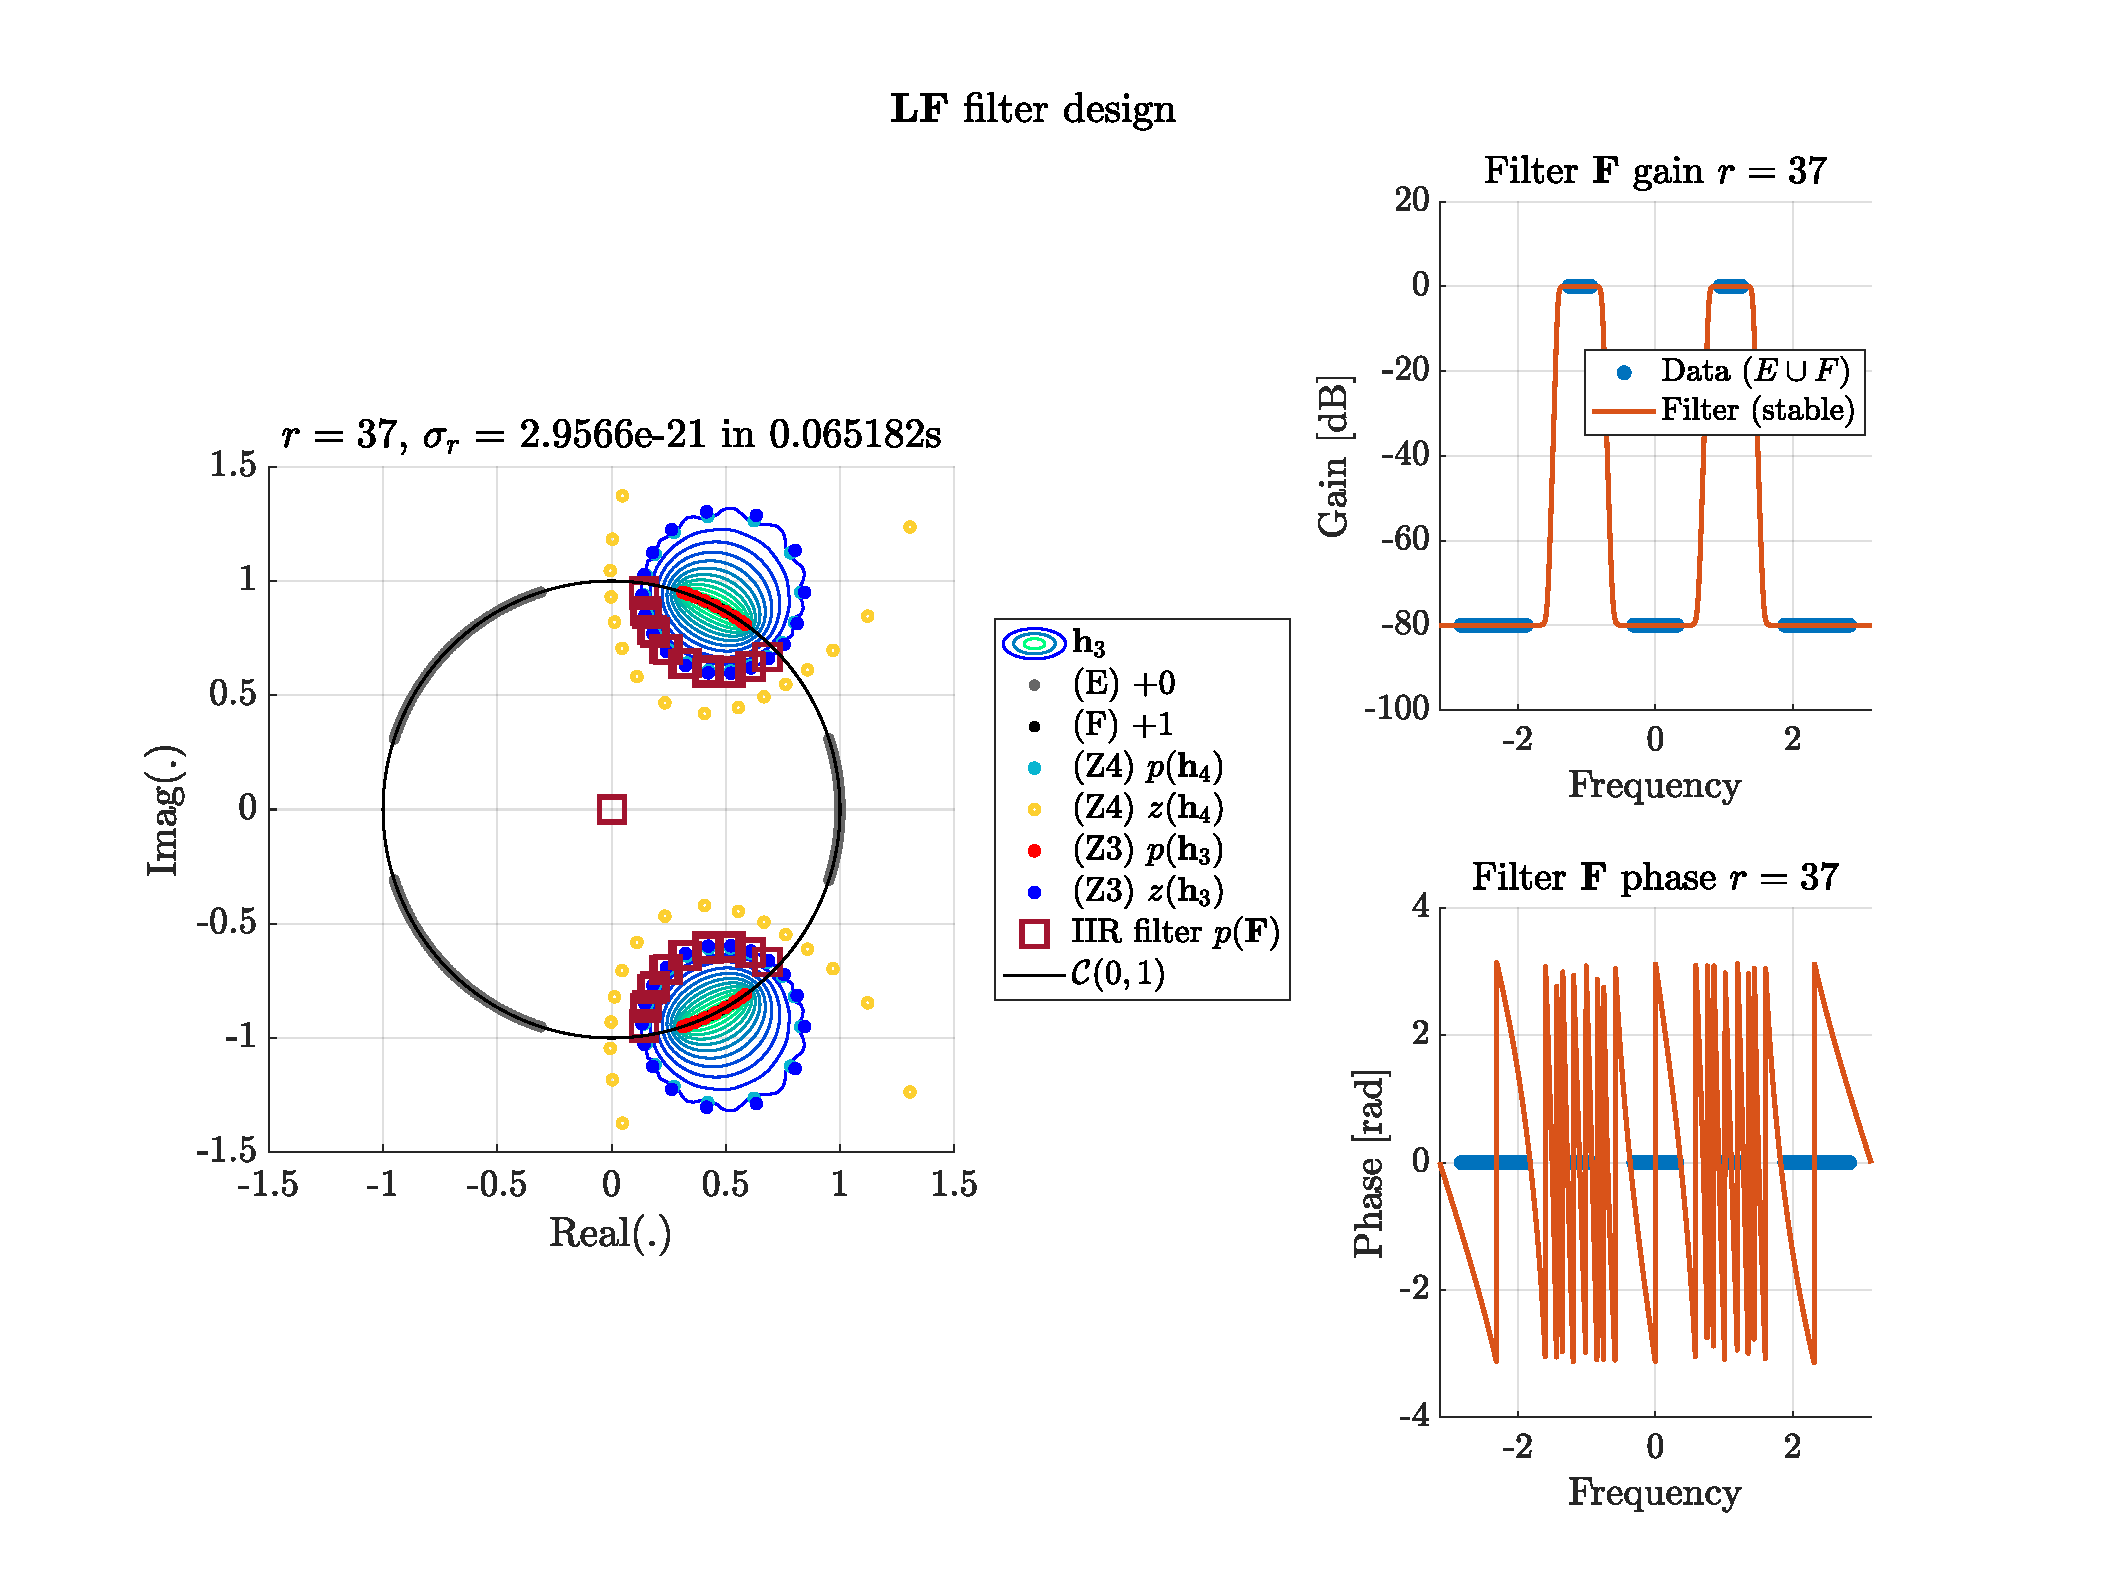
\includegraphics[width=1\textwidth]{figures/filter/iir_filter.pdf}
    \caption{Bandpass filter and connection with Z4. Left: same description as \cref{fig:intro:1a} with additionally, the mirrored poles of Z4. Right: Bode gain and phase of the obtained filter $\mathbf{F}(\varIC)$.}
    \label{fig:filter}
\end{figure}

To convince of the applicability and interest of this methodology, \cref{fig:filter_td} illustrates the application of the obtained filter $\mathbf F(\varIC)$, with a sampling time $T_s=0.2$ seconds, on a chirp signal exciting frequencies from 0 to $0.9/(2T_s)$. In \cref{fig:filter_td}, the upper part represents the time-domain response, wile the lower is the frequency-domain response obtained by FFT.

\begin{remark}[Open questions]
The above process seems very simple, yet efficient. However, some legitimate questions arise: 
\begin{itemize}
\item The projection to enforce filter $\mathbf F$ stability modifies the phase. An appropriate criterion and method should be applied to control this step. As an example, (i) a linear phase with (almost) constant time group (e.g. Bessel like), or (ii) a minimal phase variation, can be of interest.
\item The gain data fit is very good on the chosen example. However, some configurations may result with spikes in the gain at the non interpolated values, which is unlikely for filtering. Avoiding these spikes in the non-interpolated data is important and methods should be thought, e.g. (i) data completion, (ii) constraints on the derivative of $\bF(\varIC)$, or (iii) a Lawson like method for LF may be some ideas.
\end{itemize}
\end{remark}

\begin{figure}[ht]
    \centering
    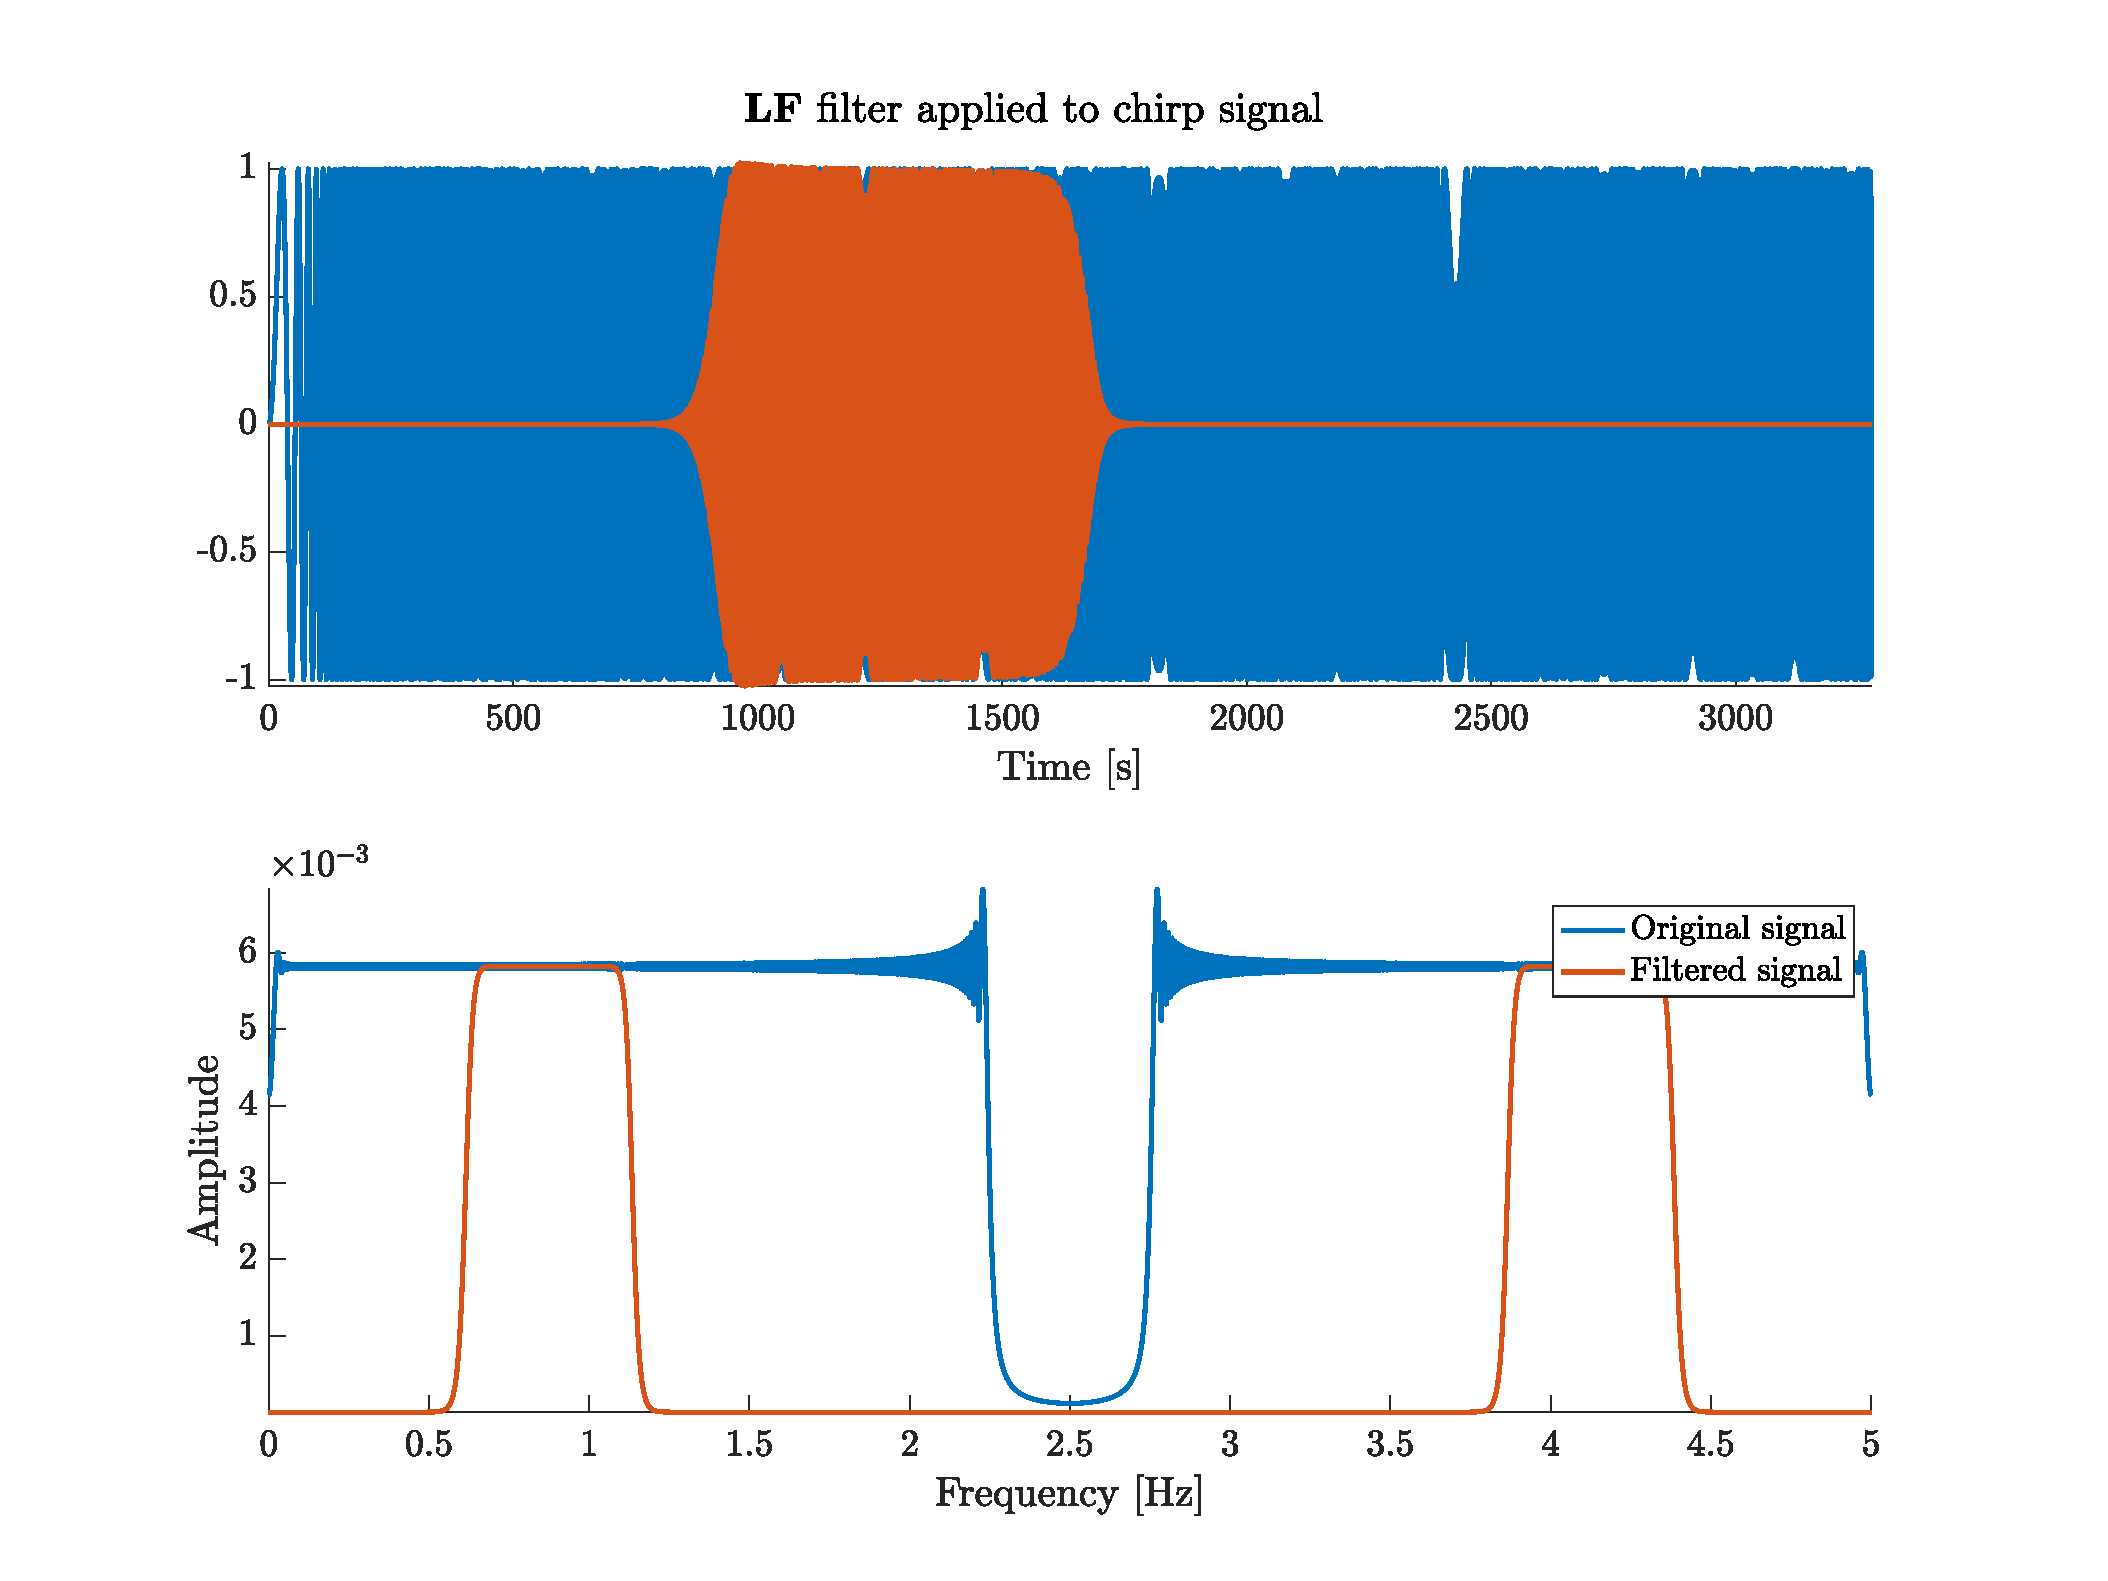
\includegraphics[width=1\textwidth]{figures/filter/iir_filter_td.pdf}
    \caption{Application of filter $\mathbf F(\varIC)$ to a chirp signal. Top frame is the time-domain responses, bottom is the associated FFT absolute value.}
    \label{fig:filter_td}
\end{figure}
